
  Les deux algorithmes implémentés ont un squelette très similaire ; il s'agit, à partir de la carte des profondeurs, de lier deux par deux les pixels de l'image générée puis de colorier chaque paire de la même couleur. L'autostéréogramme est calculé ligne par ligne de la manière suivante : pour chaque point de l'image 3D, on calcule une paire de pixels correspondant à ce point en fonction de la profondeur de l'objet en ce point. Les deux pixels d'une paire sont ensuite colorés tous deux de la même couleur. 

  Les deux algorithmes sont dotés d'une technique anti-surfaces cachées (implémentée différemment dans les deux cas), c'est-à-dire que si un point de l'objet n'est vu que par un \oe il, on ne crée pas de paire de pixels lui correspondant. Cela permet d'éviter des défauts dans l'autostéréogramme.

  Les algorithmes supportent tous deux l'utilisation de textures en plus de la génération aléatoire de pixels. 
  
  \subsubsection{Algorithme de base (Witten, Inglis, Thimbleby)}

  Cet algorithme a été choisi pour sa simplicité qui le laisse tout de même fonctionnel ; il a été conçu à l'origine pour des autostéréogrammes aléatoires en noir et blanc (SIRDS) mais a été adapté ici à d'autres types de rendus.

  Les résultats obtenus sont cependant assez peu satisfaisants pour la représentation d'objets complexes : l'objet en relief est fait de paliers superposés plutôt que d'avoir une surface lisse. De ce fait, représenter des détails ou des courbes est ardu. L'utilisation de textures peut permettre d'atténuer certains défauts visuels, mais pas de les effacer totalement.

\begin{figure}[h]
	\centering
	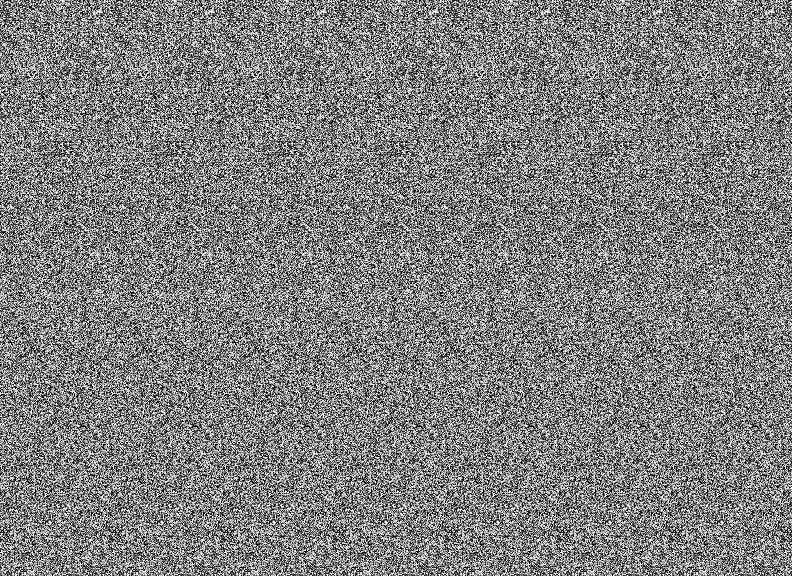
\includegraphics[scale=0.3]{autoste1.png}
	\caption{\label{fig:autoste1} Rendu d'un autostéréogramme avec l'algorithme de Witten, Inglis et Thimbleby \protect}
\end{figure}

  \subsubsection{Algorithme de W. A. Steer}
  
  L'algorithme de W. A. Steer a été choisi à cause des nombreuses améliorations qu'il apporte par rapport à l'algorithme précédent. En effet, il utilise une méthode de suréchantillonnage de l'image : dans une première étape, un autostéréogramme $n$ fois plus large que l'image de base est construit puis les pixels sont fusionnés par groupes de $n$. Ces étapes permettent d'améliorer la résolution en profondeur de l'autostéréogramme.
  
  Cet algorithme est plus lent que le précédent à cause du suréchantillonnage, mais les résultats obtenus sont nettement plus agréables à regarder car la résolution en profondeur est meilleure : l'image apparaît plus profonde comme le montre la figure \ref{fig:autoste2}. De plus, l'utilisation conjointe d'une texture et du suréchantillonage lisse l'image finale ; on n'y retrouve plus les ``paliers'' des résultats précédents. Ces paliers peuvent être visibles si le rendu choisi est de type aléatoire, mais ils sont beaucoup plus nombreux et rapprochés, donc moins évidents.

  Enfin, lors de la coloration des pixels liés, de fortes déformations de la texture de base peuvent apparaître à la gauche de l'image (en supposant que la coloration se fait de droite à gauche). Ces déformations sont d'autant plus importantes que l'objet 3D est complexe. Afin d'harmoniser l'image 2D, la coloration a ici été faite de droite à gauche dans la partie gauche de l'image, et inversement dans la partie droite.

\begin{figure}[h]
	\centering
	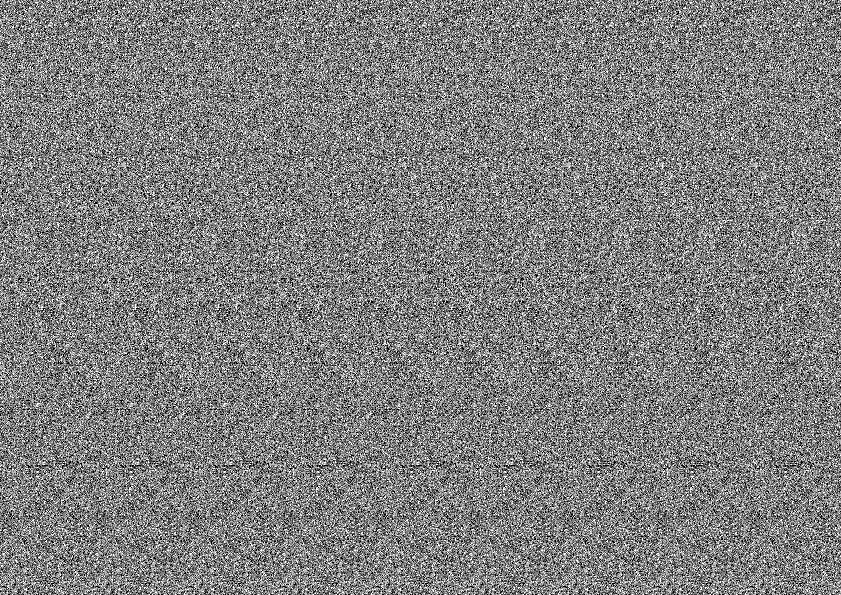
\includegraphics[scale=0.3]{autoste2.png}
	\caption{\label{fig:autoste2} Rendu d'un autostéréogramme avec l'algorithme de W. A. Steer \protect}
\end{figure}
